\documentclass{../base/base}
% Dateikodierung ist utf8
\usepackage[utf8]{inputenc}
\usepackage{url}
\usepackage[export]{adjustbox}
\usepackage{amsmath}
\usepackage{listings}
\usepackage{tikz}
\usepackage{tabularx}
\usepackage{color,colortbl}
\usepackage{ulem}
\usepackage{pdfpages}
\usepackage{ wasysym }
\usepackage{ booktabs }
\usepackage{lscape}
\usepackage{multicol}

\begin{document}

\Abgabeblatt{Assignment 3}{30.4.2018 / 07.05.2018}{????}{????}{Yannis Rohloff (yannis@uni-bremen.de)}{Meng Liu(lium@uni-bremen.de)}{Peter Tschubij (tschupet@uni-bremen.de)}

\lstset{
    language=Python,
    basicstyle=\ttfamily\small,
    aboveskip={1.0\baselineskip},
    belowskip={1.0\baselineskip},
    columns=fixed,
    extendedchars=true,
    breaklines=true,
    tabsize=4,
    prebreak=\raisebox{0ex}[0ex][0ex]{\ensuremath{\hookleftarrow}},
    frame=lines,
    showtabs=false,
    showspaces=false,
    showstringspaces=false,
    keywordstyle=\color[rgb]{0.627,0.126,0.941},
    commentstyle=\color[rgb]{0.133,0.545,0.133},
    stringstyle=\color[rgb]{01,0,0},
    numbers=left,
    numberstyle=\small,
    stepnumber=1,
    numbersep=10pt,
    captionpos=t,
    escapeinside={\%*}{*)}
}


\section*{Exercise 1: Cutting Fabric - Variable Definition}

We define our variable in a similar vein as any other coloring problem. Though it gets more complicated because shapes set constraints to neighboring parts.


Let's clarify a few terms. The \textit{workspace} is rectangular arrangement of \textit{fields}. Each \textit{fields} should be filled by one \textit{tile}, where each \textit{tile} is a part of a shape.

We consider every field on our workspace to be uniquely identified by a coordinate tuple $c = (x,y)$.
Every such field may only be occupied by one tile at a time, so that nothing overlaps. Furthermore every tile should be occupied by one tile with the exception of continuous patterns at the beginning and the end of a workspace.

A tile is represented by a 3-tuple $t = (s, r, n)$ where $m$ is the number its the shape from the input, $r$ is a number from $1$ to $4$ representing the rotation. And $n$ is the number of the tile of the shape.
We will copy every shape from the input four times to where each time w increase the $r$ accordingly.
Let $T$ be the set of all these $tiles$.

Now we can define a Variable stating if a field is occupied by a tile:
$$X_{c,s} = X_{(x,y),(s,r,n)}$$

To formulate all constraints we need to extend the workspace form the exercise. The input is a workspace of dimensions $w \cdot h$, with $h$ being the axis that can extend and w the width. No tile may be placed outside of the width.

First, we copy another workspace directly beneath the current workspace. This results in the height to double: $h := h \cdot 2$.
Let $F2$ be the set of the added fields, while $F1$ is the set of fields that existed before. And let $F = F1 \cup F2$

Second, we add another column on each side. The new width is $h := h+2$. We will use these fields to ensure that they are not \textit{painted} with a tile. Let $O$ be the set of these fields.

With $h=3,w=2$ the field looks like this. The blue fields are in $O$, the yellow fields are in $F1$ and the orange fields are $F2$. \\

\begin{center}
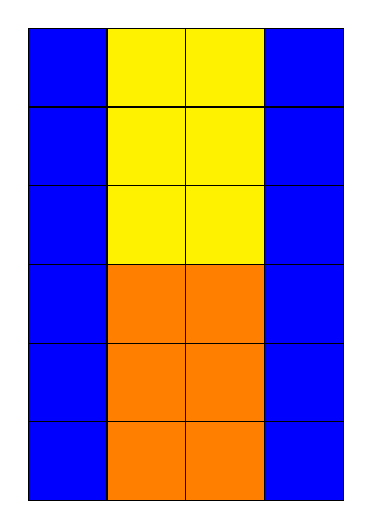
\begin{tikzpicture}[scale=1]
    \draw [fill=blue] (0,0) rectangle (1,1);
    \draw [fill=orange] (1,0) rectangle (2,1);
    \draw [fill=orange] (2,0) rectangle (3,1);
    \draw [fill=blue] (3,0) rectangle (4,1);

    \draw [fill=blue] (0,1) rectangle (1,2);
    \draw [fill=orange] (1,1) rectangle (2,2);
    \draw [fill=orange] (2,1) rectangle (3,2);
    \draw [fill=blue] (3,1) rectangle (4,2);

    \draw [fill=blue] (0,2) rectangle (1,3);
    \draw [fill=orange] (1,2) rectangle (2,3);
    \draw [fill=orange] (2,2) rectangle (3,3);
    \draw [fill=blue] (3,2) rectangle (4,3);

    \draw [fill=blue] (0,3) rectangle (1,4);:
    \draw [fill=yellow] (1,3) rectangle (2,4);
    \draw [fill=yellow] (2,3) rectangle (3,4);
    \draw [fill=blue] (3,3) rectangle (4,4);

    \draw [fill=blue] (0,4) rectangle (1,5);
    \draw [fill=yellow] (1,4) rectangle (2,5);
    \draw [fill=yellow] (2,4) rectangle (3,5);
    \draw [fill=blue] (3,4) rectangle (4,5);

    \draw [fill=blue] (0,5) rectangle (1,6);
    \draw [fill=yellow] (1,5) rectangle (2,6);
    \draw [fill=yellow] (2,5) rectangle (3,6);
    \draw [fill=blue] (3,5) rectangle (4,6);
\end{tikzpicture}
\end{center}

The reason why we duplicate the workspace is simple. We want to allow the patterns to be continuous. We assume that if a pattern only fits in a continuous it will have at least one part that is hanging over to the other workspace. Imagine we find a layout of tiles that fills the yellow area and one tile is hanging over to the orange part (top left orange field).
Constraint 4 will require the tiles in the orange and yellow area to be the same. The filled orange field now must be the same as the top left yellow field. We require all fields to be assigned to a tile resulting in a possible solution in either the yellow or the orange part (Both are the same size as the input workspace).

Overhanging shapes to the top and the bottom of the entire workspace are allowed. Additionally, if we imagine a L-Shape overhanging in a way that it would hit a blue area (if we continued the blue area) we can see that this would result in a conflict. Since both workspaces are required to be the same, the overhanging tile would be copied to an existing blue area, resulting in the conflict.




Now we can define constraints that define our problem. Some are similar those of the Graph Coloring Problem, since essentially we paint each field with a tile. 


\subsection{Constraint 1: No border has a tile.}
$$\bigwedge_{\substack{c \in O}} \bigwedge_{\substack{t \in T}} \neg X_{c,t}$$

\subsection{Constraint 2: Every field in F1 and F2 has at least one tile}
$$\bigwedge_{\substack{c \in F}} \bigvee_{\substack{t \in T }} X_{c,t}$$


\subsection{Constraint 3: Every field in F1 and F2 has at most one tile.}
$$\bigwedge_{\substack{c \in F}} \bigvee_{\substack{t1,t2 \in T \\ t1 \neq t2 }} \neg X_{c,t1} \lor \neg X_{c,t2}$$

\subsection{Constraint 4: Respective fields in and F1 and F2 have the same tiles assigned}
$$\bigwedge_{\substack{(x,y) \in F1}}\ \bigvee_{\substack{t \in T}} \neg X_{(x,y),t} \lor X_{(x,y+h),t} $$
and
$$\bigwedge_{\substack{(x,y) \in F1}}\ \bigvee_{\substack{t \in T}} \neg X_{(x,y+h),t} \lor X_{(x,y),t} $$
(Note: In our coordinate system the y axis is inverted thats why $y+h$ is below $y$)\\
(Note that you can read both as implications. Since we have both directions the implications are bidirectional)


\subsection{Constraint 5: If a tile is connected on a field, the neighbors of the field are filled with the neighbors of the tile in the shape.}

We define the sets $V$ and $H$ containing tuples of all the vertical connections and horizontal connections of tiles in a shape (Only top to bottom and left to right. They are not bidirectional).
For example: $(t1,t2) \in V$ if We have the shape:\\
.+\\
.+\\
(Note: we will rotate the input shapes four times actually we would have two tuples in H and two in V)\\

Horizontal:
$$\bigwedge_{\substack{(x,y) \in F\cup O}}\ \  \bigwedge_{\substack{(t1,t2) \in H}} \neg X_{(x,y),t1} \lor X_{(x+1,y),t2} $$
Horizontal back implication:
$$\bigwedge_{\substack{(x,y) \in F\cup O}}\ \  \bigwedge_{\substack{(t1,t2) \in H}} X_{(x,y),t1} \lor \neg X_{(x+1,y),t2} $$

Vertical:
$$\bigwedge_{\substack{(x,y) \in F\cup O}}\ \  \bigwedge_{\substack{(t1,t2) \in V}} \neg  X_{(x,y),t1} \lor X_{(x,y+1),t2} $$
Vertical back implication:
$$\bigwedge_{\substack{(x,y) \in F\cup O}}\ \  \bigwedge_{\substack{(t1,t2) \in V}} X_{(x,y),t1} \lor \neg X_{(x,y+1),t2} $$
(Note: Some of the Variables like $X_{(x,y+1)}$ don't exists. In the each case our program will ignore these clauses. We also have another theory that replacing the $\bigwedge_{\substack{(x,y) \in F\cup O}}$ in each clause by $\bigwedge_{\substack{(x,y) \in F1}}$ is sufficient, but we are not sure with that, yet.)




\end{document}
